\subsection{Methods Overview: Approach} 

We assume we have noisy observations of many `effects' in many  conditions. Our goals include estimating the sizes of the actual effects, including some measure of `significance'. In doing this we aim to exploit the fact that effects in different conditions may often be similar though not identical, while leaving open the potential to identify effects that are `specific' to only some of the conditions. Critically, we allow for subtle differences among those effects that are `similar'.  Here, we aim to learn about patterns of sharing of effects across tissues. Because these patterns are shared among SNPs, we can use the information contained in the larger data-set to help us better understand the global and snp-specific patterns of effects of genetics on gene expression. This allows us to make comparisons among tissues in which the QTL is called active, and among gene-snp pairs with a similar degree of activity in a given tissue. 

%Thus as an additional level of combining information,
Here, we assume that each eQTL may follow a particular pattern of activity characterized by its effects across tissues. Within these groups, the tissues exhibit characteristic patterns of sharing, which can be captured by considering the covariance structure of the genetic effects among tissues. This lends itself to a mixture model, in which  we assume all the gene-snp pairs arise from a mixture of a finite number of multivariate normal (MVN) distribution, each characterized by the covariance matrix from which the vector of effects is though to arise. For each of $\textbf{J}$ gene-snp pairs, we observe an R dimensional vector of standardized effect sizes %$\bm{\hat{b}}$
and their standard error and assume that these effects descend from some true effect size $\bm{b}$. 



 \begin{equation}
  \bm{b_{j}} | \bm{\pi},\bf{U} \sim \sum_{k,l} \pi_{k,l} \;{\it N}_R(.;\bm{0}, \omega_l U_{k})
  \label{eqn:mixprior}
\end{equation}

To capture both similarity and differences of effects across tissues we assume that each effect arises from one of K `types'. For example, one type could represent effects that are relatively constant across conditions (`consistent type'); and another type could represent effects that are specific to the first condition, or some other subset of conditions (i.e. are zero or close to zero in other conditions). For each type we allow that effects may come from one of $L$ `sizes'. For example, among effects that are of a `consistent' type, some may be consistently large and others may be consistently moderate.
Although we use phrases such as `consistent' and `large' here for convenience, our model allows for a range of actual quantitative values within each type-size combination (see \ref{fig:Patterns}
). Thus, effects may be active under all conditions, but with varying degrees of activity; or active with quantitative variation in a subset of conditions, and small but non-zero in other conditions. Specifically we assume that the effects $\bm{b}$ come from a mixture model (Equation \ref{eqn:mixprior}) here, where the matrix $U_{k}$  determines the similarity of effects among conditions for type k,  and the scalar $\omega_{l}$ determines the typical size of effect for size $l$. The parameters $\pi_{k,l}$ capture the relative frequency of each type-size combination, and estimating these parameters from the data is one key step in fitting this model. 

Thus the covariance matrix $U_{k}$ captures the particular patterns of sharing reflecting the variation in effect sizes within and between tissues, while $\omega_{l}$ determines the scale of each pattern - the magnitude of the effect size. The relationship among the distinct entries of this matrix allows us to specify effects which may be consistently larger in some tissues relative to others and may possess variable correlation among different pairs of tissues (e.g., see Figure \ref{fig:Patterns}, \textbf{B}, for converse relationships among effects in tissue one and two for SNPs of green opposed to blue class). Thus we also recognize that while two eQTL may obey a similar pattern or shape, the absolute scale may vary. For example, two eQTL may both have strong correlation between liver and lung with consistently larger effects in liver, but the absolute size of the effects may vary between SNPs (Figure \ref{fig:Patterns}, \textbf{A}, contrast gene-snp pairs of far left and far right pattern).Critically, these patterns are learned from the data rather than forced. 

%\textbf{Figure: Colorful patterns, caption indicates different patterns of activity across tissues in groups 1-3, same pattern or shape for snps of group 4 but tendency towards small effects}

\newline
\begin{figure}[htbp]
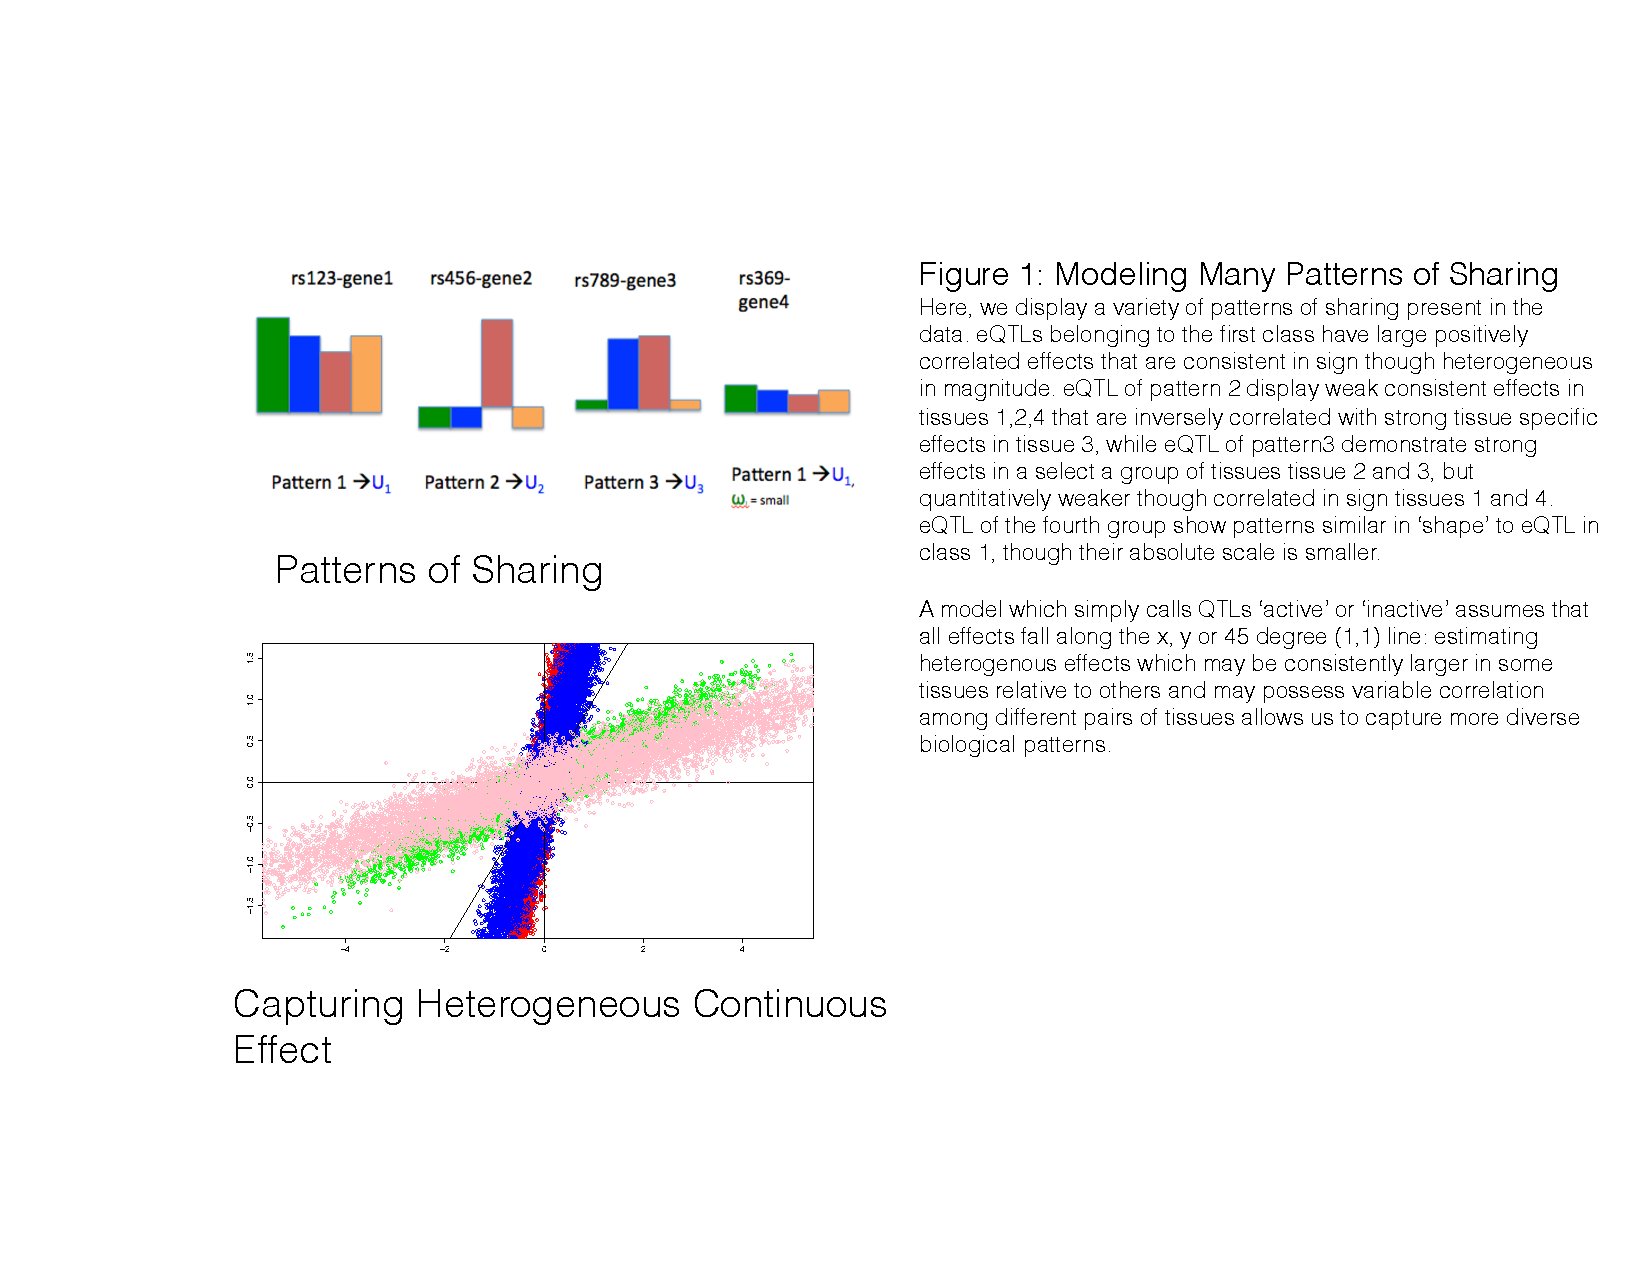
\includegraphics[width=10cm]{Figures/Patterns.pdf}%\\
%\includegraphics[width=10cm]{Figures/PlotsForPaper_files/figure-html/starterpic-1.png}
\caption{\textbf{Modeling Many Patterns of Sharing.} \textbf{A:} Here, we display a variety of patterns of sharing present in the data. eQTLs belonging to the first class have large positively correlated effects that are consistent in sign though heterogeneous in magnitude. eQTL of pattern 2 display weak consistent effects in liver, lung and thyroid that are inversely correlated with strong tissue specific effects in brain, while eQTL of pattern 3 demonstrate strong effects in a select a group of tissues (here, lung and brain), but quantitatively weaker though correlated in sign with liver and thyroid. eQTL of the fourth group show patterns similar in `shape' to eQTL in class 1, though their absolute scale is smaller. \textbf{B:} In this two tissue-example, a model which simply calls QTLs `active' or `inactive' assumes that all effects fall along the x, y or 45 degree (1,1) line: estimating heterogenous effects which may be consistently larger in some tissues relative to others and may possess variable correlation among different pairs of tissues allows us to capture more diverse biological patterns. \textbf{C:} In these examples from real data, we illustrate patterns that were `learned' from the data and demonstrate a varying range of quantitative values among tissue we've deemed active. Note $U_{k}$ 2,3 and 9 demonstrate consistent though quantitatively heterogenous effects, while patterns 4 and 5 show varying levels of tissue specificity. Contrast that with the mash-lite approach to consistency, which only allows for homogenous effects throughout.}
\label{fig:Patterns}
\end{figure}
\newline


\subsection{Previous Approach}
 
Previous work from our lab considered the idea of configuration - i.e., that a gene-snp pair was simply `active' or `inactive' in a particular tissues - and thus for R tissues, there were $2^{R}$ possible configurations, which becomes computationally infeasible as $R$ grows. Thus a non-trivial novelty of our approach is its application to joint estimation of effects across a larger number of $R$= 44 tissues, never before described.

Furthermore, this considered only the idea that the variance in effect sizes between two tissues was the same across tissues thought to be active and the covariances were also the same among tissues thought to be active in a given `configuration',  and thus failed to incorporate the much richer covariance structure between tissues. For example, many gene-SNP pairs might follow a pattern in which it is common to be `active' across all tissues, but some QTL may have consistently larger effects in liver, lung and thyroid while other QTL may possess consistently larger effects in brain tissues and still another class of gene-snp pairs may show consistently quantitatively specific activity in whole blood but non-trivial effects in other tissues. 

As a critical innovation on our previous work \cite{flutre_statistical_2013,wen_bayesian_2014} the covariance matrices used here contain distinct diagonal and off-diagonal elements which reflect data-specific patterns of variation within and covariance between subgroups (tissues). This captures the variation in effect sizes within and between subgroups better than restricting effects to simply `shared' or `unshared'. This effectively amounts to a random effects analysis in which we assume that the between subgroup variability, here the entries of the matrix $U_{k}$ is unique for each study (see Borenstein et al).

Because we can't know the `true covariance matrix' for each gene-snp pair, we aim to assemble a list which sufficiently captures the various patterns, and then `learn' the relative proportions of each pattern of sharing from the data. One can now model each vector of effect sizes $\bm{b_{j}}$ as arising from a mixture that captures all the covariance patterns present (Equation \ref{eqn:mixprior}).

The primary novelty of this approach is {\it to estimate this multivariate posterior distribution on the effect size in a data-sensitive way} - i.e., using the mixture model to capture information about the covariance structure among subgroups (here, tissues), and thus describe the heterogeneity of effects across tissues, rather than simply calling effects `shared' or `specific'. We deem this model `hierarchical' because these prevailing patterns of activity are learned from the larger dataset - e.g., a large, random set of gene-snp pairs - and influence our inference about a given gene-snp pair `$\bf{j}$'. Thus we might identify a situation in which it is common to have large effects in certain tissues and not others. Accordingly, if a given observed gene-snp pair demonstrates a small effect in one of the `off issues', we might be inclined to conclude that it is indeed a member of this particular class and shrink the small effect in this tissue accordingly without reducing our estimates of the more `active tissues'. However, if we observe the same small effect in a setting in which `similar tissues' have large effects, we might `shrink' this effect size less, due to our high prior belief in the SNP's effectiveness garnered from adjacent tissues. Thus we deem this method `Adaptive Shrinkage' because the appropriate amount of shrinkage is learned from the overall dataset. Critically, our method is dually adaptive, in the sense that we learn the relative abundance of effect sizes and directions from the overarching data set: observed effects are nudged towards prevailing patterns and sizes, according to the learned proportions of each.

Because our prior belief in consistency is strong in this particular dataset, we identify many more `significant associations'  in settings where perhaps the observed univariate statistic in one tissue is small but otherwise large in additional tissues, nudging these effects towards something more consistent. This is in contrast to a univariate shrinkage approach, in which all effects of the same size would be `shrunk' equivalently, due to lack of information garnered from adjacent tissues. 
%
%In fact, shrinkage towards $\bm{0}$ of small effects is a result, not a necessity - since the majority of the prior weight is on small $\omega$ components which emphasize components with small prior variance of the effect size $\textbm{b}$, many of the modest observed effects will be smoothed or shrunk towards the prior mean, $\bm{0}$. 

Critically, in learning about the effect size of a gene-snp pair in each tissue, we can make statements about the degree of heterogeneity present in the data-set: that is the proportion of SNPs who exhibit effects that vary in magnitude or sign. Conversely, we can describe the degree of homogeneity should these phenomena be rare. Thus we offer an additional description to eQTL analysis: the degree of heterogeneity across multiple subgroups in both sign and magnitude, by characterizing a particular QTL by the similarity in size of its effects across subgroups. 